%! Author = Patrik Skaloš

% Preamble
\documentclass[a4paper]{article}

% Packages
\usepackage[utf8]{inputenc}
\usepackage[english]{babel}
\usepackage[T1]{fontenc}
\usepackage{geometry}
\usepackage[unicode]{hyperref}
\usepackage{graphicx}
\usepackage{enumitem}

\newlist{notes}{enumerate}{1}
\setlist[notes]{label=Note: , leftmargin=2cm}


% Document
\begin{document}

  % Title page
  \begin{titlepage}
    \begin{center}

      \vspace*{5cm}

      \huge
      \textbf{A simple packet sniffer}
      
      \vspace{2cm}

      \huge
      \textbf{Patrik Skaloš}

      \vfill

      February 2022

    \end{center}
  \end{titlepage}

%%%%%%%%%%%%%%%%%%%%%%%%%%%%%%%%%%%%%%%%%%%%%%%%%%%%%%%%%%%%%%%%%%%%%%%%%%%%%%%%

  % Table of contents
  \tableofcontents

%%%%%%%%%%%%%%%%%%%%%%%%%%%%%%%%%%%%%%%%%%%%%%%%%%%%%%%%%%%%%%%%%%%%%%%%%%%%%%%%

  \newpage

  \section{Introduction}

  \subsection{Packet sniffing}

  Packet sniffing is an act of capturing frames that are being sent from or 
  received by a device on a certain network. Our program is able to capture 
  \textit{ethernet frames} on a single interface specified by the user.
  After a frame has been captured, various information about it can be printed, 
  including source and destination addresses, ports and even the encapsulated 
  data (although it is often encrypted).


  \subsection{Protocols}

  \textit{Protocols} will be mentioned many times in this document, but what 
  are they? They are simply sets of standards (rules) by which, for example, 
  data is encapsulated, transferred and so on. Without protocols, networking 
  would be a total chaos and thanks to them, it is very simple for devices to 
  read any data received since they can rely on those rules.


  \subsubsection{OSI model}
  
  To explain the protocols supported by our packet sniffer, we must first 
  introduce the OSI conceptual model of a networking system. Everything 
  important to understand can be explained by figure 1.

  \begin{figure}[h]
    \centering
    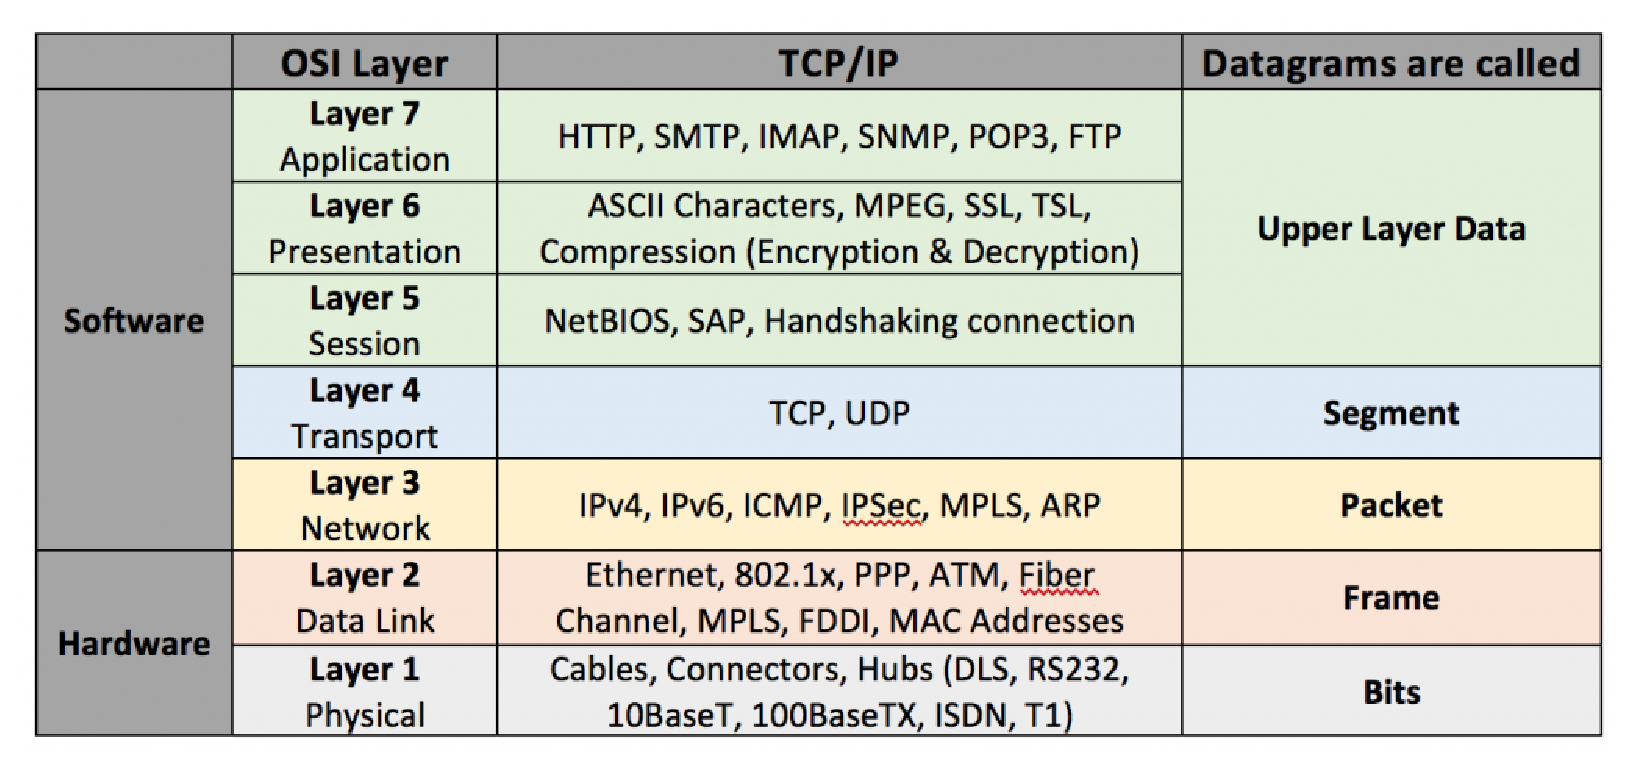
\includegraphics[width=\textwidth]{./src/osi.eps}
    \caption{OSI model \cite{techsoftcenter:osi}}
  \end{figure}


  \subsubsection{Data units}

  Before any data can be sent over a network, it has to be formatted according
  to rules that various protocols provide. We need to understand differences
  between these data units:
  \begin{itemize}
    \item Frame: encapsulates a packet
    \item Packet: encapsulates a data segment
    \item Segment: encapsulates data
  \end{itemize}
  So, for example, sending a HTTP request from the application layer means
  dividing it into several portions if it is too big, encapsulating each portion
  to a segment, then to a packet and finally to a frame before sending it 
  over a network media (e.g. cable) bit by bit.

  \begin{notes}
    \item Encapsulation means taking some data and adding metadata around it 
      (in networking, we use a header and only sometimes a trailer).
    \item Encapsulation doesn't always mean 
      \textit{data in segments in packets in frames}. Depending on a protocol,
      data, or sometimes even segments can be ommited (e.g. sending a packet 
      with no user data in it since the real value of the packet is in the 
      headers).
    \item It might be a bit confusing that a packet sniffer captures frames and
      not packets. I don't feel confident exaplaining why, but as I understand,
      word \textit{packet} is often used when referring to frames or 
      even segments and yes, to be precise, it should be called 
      \textit{frame sniffer} instead of \textit{packet sniffer}.
  \end{notes}

  \vspace{1cm}


  \subsection{Supported protocols}

  \subsubsection{Data link layer protocols}

  \textbf{Ethernet frame} is a data link layer protocol data unit in 
  which a packet is encapsulated along with MAC (physical) addresses, 
  an \textit{EtherType} field indicating which protocol is used for the packet
  and a \textit{CRC} field, which is a sequence of bits used for error 
  detection. 
  See table \ref{ethernet_frame} for visualisation. The payload field 
  represents a single packet. 
  An ethernet frame already contains all data necessary to travel over or to a 
  different network and you could say it is a data unit of the highest level.
  Ethernet frame is the only data link layer protocol supported by our packet 
  sniffer. 
  For more information, see \cite{wikipedia:ethernet_frame}.

  \begin{itemize}
    \item \textbf{Header length}: 14 bytes (112 bits)
    \item \textbf{Trailer length}: 4 bytes (32 bits)
    \item \textbf{Important header fields}:
      \begin{table}[h]
        \centering
        \begin{tabular}{|c|c|c|c|}
          \hline
          Field name & Data it represents & Field length & Field offset \\
          \hline
          \hline
          Destination MAC address & & 48 bits & 0 bits \\
          \hline
          Source MAC address & & 48 bits & 48 bits \\
          \hline
          EtherType & Protocol used in the packet & 16 bits & 96 bits \\
          \hline
        \end{tabular}
        \caption{Important ethernet frame header fields}
      \end{table}
  \end{itemize}

  \begin{table}[h]
    \centering
    \begin{tabular}{|c|c|c|c|c|}
      \hline
      Destination MAC address & Source MAC address & EtherType & 
        \textbf{Payload} & CRC \\
      \hline
    \end{tabular}
    \caption{Ethernet frame contents}
    \label{ethernet_frame}
  \end{table}

  \vspace{1cm}


  \subsubsection{Network layer protocols}

  \textbf{IPv4} (internet protocol, version 4) is the most common one and is 
  used to transfer data over the internet.
  For more information, see \cite{wikipedia:ipv4}.

  \begin{itemize}
    \item \textbf{Header length}: 20 to 60 bytes (160 to 480 bits)
    \item \textbf{Important header fields}:
      \begin{table}[h]
        \centering
        \begin{tabular}{|c|c|c|c|}
          \hline
          Field name & Data it represents & Field length & Field offset \\
          \hline
          \hline
          IHL & Header length in 32-bit words & 4 bits & 4 bits \\
          \hline
          Protocol & Protocol of the encapsulated segment & 8 bits & 72 bits \\
          \hline
          Source IP address & & 32 bits & 96 bits \\
          \hline
          Destination IP address & & 32 bits & 128 bits \\
          \hline
        \end{tabular}
        \caption{Important IPv4 packet header fields}
      \end{table}
  \end{itemize}

  \begin{notes}
    \item We need to read the header length to know how many bytes to skip to 
      get to the data, since IPv4 packet does not have a fixed header length.
    \item We don't need the version field as we already know the internet 
      protocol version thanks to the \textit{EtherType} field of the ethernet 
      frame.
  \end{notes}

  \vspace{1cm}


  \textbf{IPv6} (internet protocol, version 6) is very similar to IPv4. It is
  supposed to be an improvement because IPv6 provides much larger
  address space as it's addresses are 128 bits long, while IPv4 addresses 
  are only 32 bits long.
  For more information, see \cite{wikipedia:ipv6}.

  \begin{itemize}
    \item \textbf{Header length}: 40 bytes (320 bits)
    \item \textbf{Important header fields}:
      \begin{table}[h]
        \centering
        \begin{tabular}{|c|c|c|c|}
          \hline
          Field name & Data it represents & Field length & Field offset \\
          \hline
          \hline
          Next Header & equivalent to \textit{Protocol} field of IPv4 & 8 bits & 48 bits \\
          \hline
          Source IP address & & 128 bits & 64 bits \\
          \hline
          Destination IP address & & 128 bits & 192 bits \\
          \hline
        \end{tabular}
        \caption{Important IPv6 packet header fields}
      \end{table}
  \end{itemize}

  \vspace{1cm}


  \textbf{ICMP} (internet control message protocol) is used by devices for
  diagnostics and reporting errors. According to my research, ICMP packet is 
  not encapsulated in an IP packet in any way (evidence lies in the fact that 
  it is a network layer protocol, not transport layer protocol. However, ICMP 
  packet could be represented as an union of IP header, ICMP header and data, 
  since the beginning of the ICMP header is the same as an IP header.
  For more information, see \cite{wikipedia:icmp}.

  \begin{notes}
    \item Command \textit{ping} uses ICMP.
  \end{notes}

  \begin{itemize}
    \item \textbf{Header length}: 8 bytes (32 bits)
    \item \textbf{Important header fields}:
      \begin{table}[h]
        \centering
        \begin{tabular}{|c|c|c|c|}
          \hline
          Field name & Data it represents & Field length & Field offset \\
          \hline
          \hline
          Type & Message type & 8 bits & 0 bits \\
          \hline
          Code & Message code (subtype) & 8 bits & 8 bits \\
          \hline
        \end{tabular}
        \caption{Important ICMP header fields (without the IP part)}
      \end{table}
  \end{itemize}

  \vspace{1cm}


  \textbf{ARP} (address resolution protocol) is a protocol used by devices to 
  keep track of IP addresses associated with MAC addresses of devices in a 
  given network. These associations are kept in a so-called \textit{ARP table}.
  The packet originates on the network layer itself. A single ARP packet can 
  represent an ARP request or an ARP response.
  For more information, see \cite{wikipedia:arp}.

  \begin{itemize}
    \item \textbf{Header length}: 8 bytes (64 bits)
    \item \textbf{Important packet fields}:
      \begin{table}[h]
        \centering
        \begin{tabular}{|c|c|c|c|}
          \hline
          Field name & Data it represents & Field length & Field offset \\
          \hline
          \hline
          OPCODE & Indicating a request or a reply & 16 bits & 48 bits \\
          \hline
          Source MAC address & & 48 bits & 64 bits \\
          \hline
          Source protocol address & Sender IP address & 32 bits & 112 bits \\
          \hline
          Target MAC address & & 48 bits & 144 bits \\
          \hline
          Target protocol address & Target IP address & 32 bits & 192 bits \\
          \hline
        \end{tabular}
        \begin{notes}
          \item Protocol address lengths (and therefore offsets) might be 
            inaccurate since different sources tell different numbers
        \end{notes}
        \caption{Important ARP packet fields}
      \end{table}
  \end{itemize}

  \vspace{1cm}


  \subsubsection{Transport layer protocols}

  \textbf{TCP} (transmission control protocol) is the most common transport 
  layer protocol. It provides a reliable way to send and receive data over a 
  network and it directly encapsulates a raw segment of data by adding 
  a TCP header to it. 
  The main aspects of the TCP are:
  \begin{itemize}
    \item Before any data is sent, a three-way handshake is used 
      to initialize the network connection between two nodes (devices)
    \item If a packet is lost or damaged (data received does not match the 
      data sent) on the way, it is retransmitted. This is to make sure
      that all packets arrive to the destination perfectly fine
  \end{itemize}
  This process is great, but as you can imagine, this increases the latency 
  since the handshake and error-checking takes time and frames have to be 
  bigger.
  For more information, see \cite{wikipedia:tcp}.

  \begin{itemize}
    \item \textbf{Header length}: 20 to 60 bytes (160 to 480 bits)
    \item \textbf{Important header fields}:
      \begin{table}[h]
        \centering
        \begin{tabular}{|c|c|c|c|}
          \hline
          Field name & Data it represents & Field length & Field offset \\
          \hline
          \hline
          Source port & & 16 bits & 0 bits \\
          \hline
          Destination port & & 16 bits & 16 bits \\
          \hline
          Sequence number & & 32 bits & 32 bits \\
          \hline
          Acknowledgement number & & 32 bits & 64 bits \\
          \hline
          Data offset & Header length in 32-bit words & 4 bits & 96 bits \\
          \hline
          Flags & & 8 bits & 104 bits \\
          \hline
        \end{tabular}
        \caption{Important TCP segment header fields}
      \end{table}
  \end{itemize}

  \vspace{1cm}


  \textbf{UDP} (user datagram protocol) on the other hand 
  \textit{does not care if the packets get damaged or lost} which increases
  the communication speed. No handshake is done and communication uses a simple
  \textit{request-response} method. This protocol is however unsuitable for most 
  applications and is used mainly for audio and video streaming (large files
  where speed matters and minor damages to packets are acceptable).
  For more information, see \cite{wikipedia:udp}.
  \begin{notes}
    \item UDP segments are also called datagrams.
  \end{notes}

  \begin{itemize}
    \item \textbf{Header length}: 8 bytes (64 bits)
    \item \textbf{Important header fields}:
      \begin{table}[h]
        \centering
        \begin{tabular}{|c|c|c|c|}
          \hline
          Field name & Data it represents & Field length & Field offset \\
          \hline
          \hline
          Source port & & 16 bits & 0 bits \\
          \hline
          Destination port & & 16 bits & 16 bits \\
          \hline
        \end{tabular}
        \caption{Important UDP segment header fields}
      \end{table}
  \end{itemize}

  \newpage

%%%%%%%%%%%%%%%%%%%%%%%%%%%%%%%%%%%%%%%%%%%%%%%%%%%%%%%%%%%%%%%%%%%%%%%%%%%%%%%%

  \section{Implementation}

  \subsection{Networking libraries used}

  This is a list of networking libraries used and some of functions or 
  structures they provide:
  \begin{itemize}
    \item \verb|pcap.h| provides several important functions for discovering
      available interfaces and using them
    \item \verb|arpa/inet.h| provides \verb|inet_ntop| function used to 
      convert IP addresses to strings, \verb|ntohs| and \verb|ntohl|
      functions to parse header data in case of different network and host 
      \verb|endianness|
    \item \verb|netinet/ether.h| provides \verb|ether_header| structure
      that an ethernet header can be typecasted to
    \item \verb|netinet/ip6.h| provides \verb|ip6_hdr| structure
    \item \verb|netinet/tcp.h| provides \verb|tcp_hdr| structure
    \item \verb|netinet/ip_icmp.h| provides \verb|ip| and \verb|icmphdr|
      structures
  \end{itemize}


  \subsection{Capabilities and limitations}

  Supported data link layer protocols:
  \begin{itemize}
    \item Ethernet (our sniffer only captures Ethernet frames)
  \end{itemize}

  \noindent
  Supported network layer protocols:
  \begin{itemize}
    \item IPv4
    \item IPv6
    \item ICMP
    \item ARP
  \end{itemize}

  \noindent
  Supported transport layer protocols:
  \begin{itemize}
    \item TCP
    \item UDP
  \end{itemize}


  \subsection{Execution}

  \begin{verbatim}
  ./ipk-sniffer [-h] [-i int] [-p port] [--tcp] [--udp] [--arp] [--icmp] 
      [-n num]

  -h print this help
  -i interface to sniff on
  -p port to use
  --tcp, --udp, --icmp, --arp select protocols to filter the traffic by.
    If none is used, all four protocols are selected by default
  -n amount of packets to stop after

  Note: Program may require root privileges
  \end{verbatim}


  \subsubsection{Examples}

  \noindent
  \textbf{Print usage}
  \begin{verbatim}
    ./ipk-sniffer -h
  \end{verbatim}

  \noindent
  \textbf{Print all available interfaces}
  \begin{verbatim}
    ./ipk-sniffer -i
  \end{verbatim}

  \noindent
  \textbf{Listen on interface wlo1 for 4 TCP frames}
  \begin{verbatim}
    ./ipk-sniffer -i wlo1 --tcp -n 4
  \end{verbatim}

  \noindent
  \textbf{Listen on interface wlo1 for any one frame on port 80}
  \begin{verbatim}
    ./ipk-sniffer -i wlo1 -p 80
  \end{verbatim}

  \noindent
  \textbf{Listen on interface wlo1 for an ICMP frame or  UDP frame on port 80}
  \begin{verbatim}
    ./ipk-sniffer -i wlo1 -p 80 --udp --icmp
  \end{verbatim}


  \subsection{Output format}

  \subsubsection{Data printed about all captured frames:}
    
  \begin{verbatim}
  timestamp:               YYYY-MM-DDThh:mm:ss.uuuuuuZ
  src MAC:                 xx:xx:xx:xx:xx:xx
  dst MAC:                 xx:xx:xx:xx:xx:xx
  frame length:            N bytes
  network layer proto:     PROTOCOL

  WHOLE_FRAME_AS_BYTES_AND_CHARACTERS
  \end{verbatim}
  \begin{notes}
    \item \textit{DATA} is printed at the end of the report. For more 
      information see \ref{section:data_format}
  \end{notes}


  \subsubsection{Additional data printed depending on the packet protocol}

  \noindent
  \textbf{ARP}:
  \begin{verbatim}
  operation:               request/reply/unknown: CODE
  src MAC:                 xx:xx:xx:xx:xx:xx
  src IP:                  IP_ADDRESS
  tgt MAC:                 xx:xx:xx:xx:xx:xx
  tgt IP:                  IP_ADDRESS
  \end{verbatim}

  \noindent
  \textbf{ICMP}:
  \begin{verbatim}
  transport layer proto:   PROTOCOL
  src IP:                  IP_ADDRESS
  dst IP:                  IP_ADDRESS
  msg type:                N
  msg code:                N
  \end{verbatim}

  \noindent
  \textbf{IP}:
  \begin{verbatim}
  transport layer proto:   PROTOCOL
  src IP:                  IP_ADDRESS
  dst IP:                  IP_ADDRESS
  src port:                N
  dst port:                N
  \end{verbatim}


  \subsubsection{Additional data printed depending on the segment protocol}

  \noindent
  \textbf{TCP}:
  \begin{verbatim}
  seq number:              N
  ack number:              N
  flags as bits:           bbbbbbbb
  \end{verbatim}

  \noindent
  \textbf{UDP}:
  none


  \subsubsection{Data format}
  \label{section:data_format}


  Data is printed at the end of a report of a captured frame and prints the 
  entire frame as bytes and characters in the following format:
  \begin{verbatim}
  OFFSET_IN_HEX: 16_BYTES_IN_HEX_SEPARATED_BY_SPACES 16_BYTES_AS_CHARACTERS
  \end{verbatim}
  Example:
  \begin{verbatim}
  0x0000: 17 03 03 00 39 64 b2 55  4f e8 4f ba 40 6c 97 32  ....9d.U O.O.@l.2
  0x0010: 66 d1 cd 7b 11 3e 3c 13  0d 58 67 8a bc 77 ee 71  f..{.><. .Xg..w.q
  0x0020: 31 b9 75 97 8e 47 1b 94  2d 8c cd de 22 51 13 81  1.u..G.. -..."Q..
  0x0030: b1 8a 98 0b 7c a6 09 bb  ee 3d f3 17 80 d3        ....|... .=....
  \end{verbatim}


  \subsubsection{TCP segment output example}

  \begin{verbatim}
  timestamp:               2022-03-01T08:18:59.210383Z
  src MAC:                 00:05:96:1f:4e:30
  dst MAC:                 ac:67:5d:1a:fa:89
  frame length:            68 bytes
  network layer proto:     IPv4
  transport layer proto:   TCP
  src IP:                  168.119.79.28
  dst IP:                  147.299.189.109
  src port:                1
  dst port:                208
  seq number (raw):        427943615
  ack number (raw):        3390744016
  flags as bits:           00011000

  0x0000: ac 67 5d 4f fa 83 00 04  96 1d 4e 30 08 00 45 a4  .g]O.... ..N0..E.
  0x0010: 00 34 42 6b 40 00 38 06  5e b0 97 65 c1 45 93 e5  .4Bk@.8. ^..e.E..
  0x0020: b4 74 01 bb e5 46 bb 9a  09 94 74 f6 da cb 80 10  .t...F.. ..t.....
  0x0030: 01 25 48 84 00 00 01 01  08 0a fb 5d d5 82 b3 1a  .%H..... ...]....
  0x0040: 0c 21 00 ff                                       .!..
  \end{verbatim}


  \subsection{Notes on my implementation}

  \begin{itemize}
    \item Since the \verb|getopt.h| library isn't very supportive of long 
      options with a value (for example \verb|--intefrace name|), I had to give
      up checking the \verb|opterr| variable to see if any errors occured while
      parsing the options. However, I don't see this being that big of a deal.
    \item When printing data, I print bytes until the end of the frame 
      indicated by \verb|caplen| variable contained in a \verb|pcap_pkthdr|
      structure returned by \verb|pcap_next| function (this function is the one
      that captures frames and returns the mentioned header and a pointer to 
      the frame as a sequence of bytes). The problem is that I couldn't find 
      any information about whether the \verb|caplen| is calculated including 
      the \verb|CRC| field (Ethernet frame trailer) length or not. I assume 
      that reading all the way to \verb|caplen| is the right way since I 
      tested it and often received meaningful printable characters as the last 
      bytes. This, however, does not make much sense and at first, I was 
      certain I should trim the last 4 bytes (\verb|CRC| length).
    \item To provide a safe way to kill the server using the \verb|SIGINT| 
      signal at any time (e.g. using \verb|Control+C|), we are capturing said 
      signal and before exiting, \textit{freeing} all resources.
    \item I understand that addresses and such contained in a frame can be 
      encoded using a different \textit{endianness} than our computers use
      and they often need to be converted. Luckily, \verb|arpa/inet.h| provides
      \verb|ntohs| and \verb|ntohl| functions to convert a short integer (16 
      bits) or a long integer (32 bits) from the network \textit{endianness} 
      to the host \textit{endianness}. However, by testing I found out it 
      should not be applied to \textbf{all} the header fields longer than 2 
      bytes. So the question has to be asked: when exactly should I use the 
      \verb|ntohs| or \verb|ntohl| functions to read data from a frame? The
      closest thing to an answer was to use it on any header field with
      length bigger than a byte, which is, obviously, not specific enough. The
      way I handled this issue was using said functions everywhere and 
      testing\,--\,in case the program was printing incorrect values, I removed
      the converting function call and tested again to see if it helped.
    \item There is a function called \verb|inet_ntoa| in the \verb|arpa/inet.h|
      library which can be used to convert a MAC address to a string. This was 
      however not suitable as it trimmed any leading zeros and prints
      \verb|0:0:3:ab...| instead of \verb|00:00:03:ab...|. Luckily, there is
      a simple (although a bit ugly ugly) way to print it without this function 
      in just four lines (although, it uses \verb|printf| which is not very 
      \textit{C++-like}).
  \end{itemize}


  \subsection{Testing}

  \subsubsection{Testing on Ubuntu 20.04.4 LTS - personal computer}
  
  First tests were performed on my personal computer and while I initially
  tested using commands like \verb|curl|, \verb|ping| and such, the real
  testing only began after I installed and opened \verb|wireshark|. I
  tried all possible combinations of supported protocols and compared my 
  outputs to the \verb|wireshark|'s outputs. It was a bit tricky to find the 
  pair to compare a single frame with but it was totally worth it. Although, I 
  was able to isolate TCP packets by using a simple HTTP server on a custom 
  port. Doing that, I found several mistakes as displaying ports, IPv6 
  addresses and even the timestamps (I was displaying microseconds in a 
  hexadecimal format).


  \subsubsection{Testing on Ubuntu 20.04.2 LTS - reference virtual machine}

  I didn't expect that testing on the reference virtual machine would be 
  unsuccessful due to it being pretty much the same operating system as on my
  personal computer, but I tested there anyways. I tested ARP, ICMP, TCP and 
  UDP protocols but could not test IPv6 capabilities, because the virtual 
  machine (or \verb|VirtualBox| or whatever else) does not support it. Anyways,
  all tests were successful.

  \begin{figure}[h]
    \includegraphics[width=\textwidth]{./src/testing.eps}
    \caption{Testing on \textit{Ubuntu 20.04.2 LTS} using \textit{Wireshark}}
  \end{figure}

  \newpage

%%%%%%%%%%%%%%%%%%%%%%%%%%%%%%%%%%%%%%%%%%%%%%%%%%%%%%%%%%%%%%%%%%%%%%%%%%%%%%%%

  \section{Conclusion}

  Programming a packet sniffer in C++ is not as hard as I initially thought
  thanks to all the libraries that help us parse datagram headers. The most
  important things are to understand the OSI model layers and protocols and 
  datagrams associated with those layers, to not forget to convert from the 
  network \textit{endianness} using \verb|htons| and \verb|htonl| and to know
  about the available networking libraries that save us a ton of work. That
  is not to say that the project was easy. Understanding the layers and 
  protocols took a lot of time and some things still confuse me or I am still 
  not sure about (e.g. what exactly is the relationship between the ICMP and IP
  protocols).

  \newpage

%%%%%%%%%%%%%%%%%%%%%%%%%%%%%%%%%%%%%%%%%%%%%%%%%%%%%%%%%%%%%%%%%%%%%%%%%%%%%%%%

  % Include bibliography
  \bibliographystyle{plain}
  \bibliography{bibliography}

\end{document}
